\subsubsection*{12.}
Pour afficher les roles d'admin on va utiliser la table USER\_ROLE\_PRIVS et just afficher 
l'attribut granted\_name (nom du role) depuis admin

\lstinputlisting[style=sqlstyle]{SQL/Partie5/role.sql}

\begin{center}
    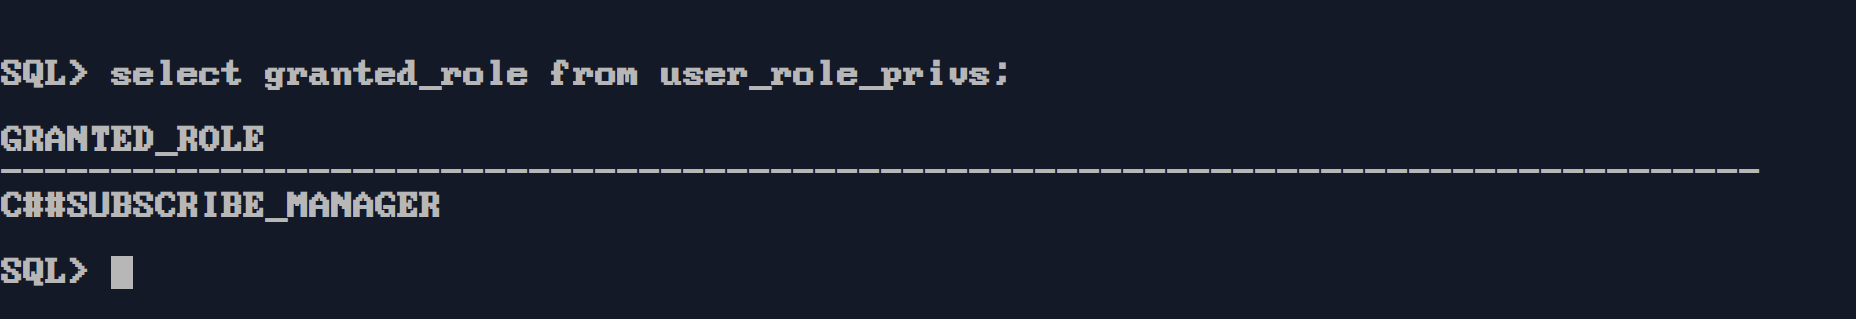
\includegraphics[width=\textwidth]{ScreenShot/Partie5/role.png}
\end{center}

\begin{prettyBox}{Remarque}{myblue}
Le role C\#\#SUBSCRIBE\_MANAGER a ete creer dans la partie4
\end{prettyBox}
